%%%%%%%%%%%%%%%%%%%%%%%%%%%%%%%%%%%%%%%%%%%%%%%%%%%%%%%
% This is a template for the Cardiff University, Doctoral Thesis 
% Viviana Greco   
% October 2023
%%%%%%%%%%%%%%%%%%%%%%%%%%%%%%%%%%%%%%%%%%%%%%%%%%%%%%%

%Font size should be no less than 12 point
\documentclass[12pt,oneside]{book}

% Margins
\usepackage{vmargin}
\setmarginsrb           { 1.5in}  % left margin
                        { 0.6in}  % top margin
                        { 1.0in}  % right margin
                        { 0.8in}  % bottom margin
                        {  20pt}  % head height
                        {0.25in}  % head sep
                        {   9pt}  % foot height
                        { 0.3in}  % foot sep

% Line Spacing
\usepackage{setspace}
\doublespacing % For double line spacing

% Paragraph Settings
\usepackage{parskip} % Import parskip package for paragraph formatting
\setlength{\parskip}{\baselineskip} % Set the space between paragraphs to be equal to one line height
\setlength{\parindent}{0pt} % Set paragraph indentation to zero

% Captions and Footnotes Font Size
\usepackage[font={normalsize}]{caption} % Import caption package to customize caption fonts
\captionsetup{
    format=plain,           % Set caption format to plain (default: hanging)
    singlelinecheck=false,  % Force alignment to justify, even for single line captions
    font={normalsize}       % Set caption font size to normal size (12pt by default)
}

% Page Header and Footer Settings
\usepackage{fancyhdr}      % Import fancyhdr package to customize headers and footers
\fancyhf{}                 % Clear all header and footer fields
\fancyhead[R]{\leftmark}   % Set right header to display the current chapter/section name
\fancyfoot[C]{\thepage}    % Set center footer to display the current page number
\renewcommand{\headrulewidth}{0.4pt} % Set the header rule width to 0.4pt

% Adjustbox Package
\usepackage{adjustbox} % Import adjustbox for flexible resizing and alignment of boxes

% Bigints Package for Large Integral Signs
\usepackage{bigints} % Import bigints for displaying large integral signs

% Placeins Package for Float Barriers
\usepackage{placeins} % Import placeins for controlling float placement
% \FloatBarrier command can be used to ensure all floats (figures/tables) are processed before continuing

\usepackage{tocloft} % Import tocloft for customizing the Table of Contents, List of Figures, etc.
% Define how figures are listed in the List of Figures (LoF)
\renewcommand{\cftfigpresnum}{\figurename~} % Prefix figure name (e.g., "Figure") before the number in LoF
\renewcommand{\cftfigaftersnum}{:} % Add colon after the figure number in LoF
\newlength{\mylen} % Create a new length variable
\settowidth{\mylen}{\cftfigpresnum\cftfigaftersnum} % Measure the width of the prefix and colon
\addtolength{\cftfignumwidth}{\mylen} % Adjust the width for figure number in LoF to accommodate prefix and colon

% Babel Package for Multilingual Support
\usepackage[english]{babel} % Import babel with English language for multilingual support and hyphenation

% Graphics
\usepackage{tikz} % Import tikz for creating complex diagrams and graphical elements
\usepackage{graphicx} % Import graphicx to provide the \includegraphics command for adding images to the document

\usepackage{stackengine} % Import stackengine for vertically stacking objects such as symbols or images

% Helvet Package for Arial Font
\usepackage{helvet} % Import helvet package to use Arial font

% AMSMath Package for Enhanced Math Features
\usepackage{amsmath} 

% Float Package for Improved Float Handling
\usepackage{float} 

% Tables
\usepackage{threeparttable}  % Import threeparttable for tables with a structured note section below the table
\usepackage{threeparttablex} % Import threeparttablex for extending threeparttable functionalities to long tables created with longtable package
\usepackage{multicol}        % Import multicol for using multiple columns in the document layout
\usepackage{multirow}        % Import multirow for creating table cells spanning multiple rows
\usepackage{longtable}       % Multi-page tables
\usepackage{booktabs}        % Import booktabs for creating professional-quality tables with enhanced layout and design

% SIUnitx Package for SI Units
\usepackage{siunitx} % Import siunitx for proper typesetting of SI units, aligning numbers in tables, and other numeric data features



% Font Encoding Packages
\usepackage[T1]{fontenc} % Import fontenc with T1 encoding for better font rendering and support for European characters
\usepackage[utf8]{inputenc} % Import inputenc with UTF-8 encoding for supporting a wide range of input characters

% CSQuotes for Context-Sensitive Quotation Marks
\usepackage{csquotes} 
% Hyperref allows to create links. Load with option to make them black
\usepackage[colorlinks=true, allcolors=black]{hyperref}

% BibLaTeX for Bibliography Management
\usepackage[backend=biber, style=apa]{biblatex} % Import biblatex with Biber backend and APA style for advanced bibliography management
\addbibresource{references.bib}
\DefineBibliographyStrings{english}{%
  bibliography = {References},
}

% \usepackage{showframe} %is any content spilling out?


%%%%%%%%%%%%%%%%%%%%%%%%%%%%%%%%%%%%%%%%%%%%%%%%%%%%%%%%%%%%%%%%%%%%%%%%%%%%%%%%%%%%%%%%%%%%%%%%%

%START
\begin{document}

% Sets numbering division level for TOC
\setcounter{secnumdepth}{4}  % Numbering depth to subsubsection
\setcounter{tocdepth}{4}  % Include depth to subsubsection in ToC

% Front matter (Title page, thesis summary, acknowledgment etc.)
\pagestyle{empty} % no headers in this section
\begin{titlepage}
\vspace*{\fill}

% Horizontal centering
\begin{center}

	\Huge
	{\textbf{Exploring Non-Invasive Methods to Improve Cognition via Sleep Manipulation}}
 	
 	\vspace{2cm}
     \begin{minipage}[c][4.5cm][c]{\textwidth}
        \centering     
		
\includegraphics[height=4cm]{./0_Front_matter/graphics - front matter//Cardiff Uni Logo.png}%
	\end{minipage}%

    \vspace{1cm}
    \large \textbf{Viviana Greco\\}
 
	\vspace{3cm}
 
	\begin{minipage}{0.9\textwidth} 
    \centering % Center the content within the minipage
	A Thesis submitted for the degree of Doctor of Philosophy
 
	\vspace{1cm}
    \large {Cardiff University\\}
    	\vspace{0.2cm}
    \large {School of Psychology\\}
    	\vspace{0.2cm}
    \large {October 2023\\}

	
    \end{minipage}
    \end{center}


\vspace*{\fill}

		

\end{titlepage}
 % Title page inside of the book
\begin{onehalfspacing} 
\frontmatter
% First blank page
\newpage
\thispagestyle{empty}
\mbox{}

% Second blank page
\newpage
\thispagestyle{empty}
\mbox{}

% Third blank page
\newpage
\thispagestyle{empty}
\mbox{}

\pagestyle{plain} % Set the page style to 'plain' for subsequent pages
\markboth{}{}
\chapter{Thesis summary}
On average, we spend one-third of our lives asleep, and we have little idea why. 
Despite the importance of sleep to overall health, sleep has been neglected for decades and considered an inactive state in which the brain “turns off” to rest from daily activities. However, there is now compelling evidence that sleep plays a pivotal role in various domains, including learning and memory, physical and mental wellbeing. The work described in this thesis is centred around exploring non-invasive ways of manipulating sleep to enhance cognition. 

\textbf{Chapter 2} delves into the effects of wearing an eye mask to block out light during sleep and its implications for daily life. This simple and cost-effective manipulation resulted in enhanced reaction times and better memory encoding compared to a control condition. Such improvements are particularly advantageous in situations demanding rapid reflexes, like driving. Furthermore, the benefits can extend to academic and professional spheres, leading to enhanced performance across diverse tasks.

\textbf{Chapter 3} investigates whether sleep facilitates insight problem solving. We found that offline consolidation and reorganisation of memories had a beneficial effect on insight, but this result was confounded by the influence of circadian rhythms.

Finally,\textbf{ Chapter 4} explores the potential benefits of an experimental technique called targeted memory reactivation (TMR) applied during rapid eye movement (REM) sleep for arousal processing. Our manipulation resulted in a reduction of emotional reactivity, as demonstrated by objective measurements of arousal.  Notably, the effect of cueing on subjective arousal responses was tied to participants’ baseline arousal levels. 

In conclusion, this thesis provides valuable insights into the importance of sleep in enhancing cognitive functions and sheds light on non-invasive interventions whose implications extend far beyond the laboratory and into everyday life.

\newpage
\thispagestyle{plain} %% add page number to blank pages
\mbox{}

\markboth{}{}
\chapter*{Declaration and Statements}
\addcontentsline{toc}{chapter}{Declaration and Statements}\label{chapter:Declaration and Statements}
\textbf{Declaration}\\
This thesis is the result of my own independent work, except where otherwise stated, and the views expressed are my own. Other sources are acknowledged by explicit references. The thesis has not been edited by a third party beyond what is permitted by Cardiff University's Use of Third Party Editors by Research Degree Students Procedure.

Signed: \stackon{\rule{1.5in}{.55pt}}{Viviana Greco} Date: 09/10/2023


\textbf{Statement 1}\\
This thesis is being submitted in partial fulfilment of the requirements for the degree of PhD.

Signed: \stackon{\rule{1.5in}{.55pt}}{Viviana Greco} Date: 09/10/2023

\textbf{Statement 2}\\
This work has not been submitted in substance for any other degree or award at this or any other university or place of learning, nor is it being submitted concurrently for any other degree or award (outside of any formal collaboration agreement between the University and a partner organisation).

Signed: \stackon{\rule{1.5in}{.55pt}}{Viviana Greco} Date: 09/10/2023

\textbf{Statement 3}\\
I hereby give consent for my thesis, if accepted, to be available in the University’s Open Access repository (or, where approved, to be available in the University's library and for inter-library loan), and for the title and summary to be made available to outside organisations, subject to the expiry of a University-approved bar on access if applicable.

Signed: \stackon{\rule{1.5in}{.55pt}}{Viviana Greco} Date: 09/10/2023

WORD COUNT: 31153\\
(Excluding summary, acknowledgements, declarations, contents pages, appendices, tables, diagrams and figures, references, bibliography, footnotes and endnotes).
\newpage
\thispagestyle{plain} %% add page number to blank pages
\mbox{}
\newpage
% Produce table of contents
\tableofcontents

\markboth{}{}
\chapter*{Acknowledgements}
\addcontentsline{toc}{chapter}{Acknowledgements}\label{chapter:acknowledgments}

At the end of this path, I would like to express my sincere gratitude to those who have played instrumental roles in my journey.

First and foremost, my deepest gratitude goes to \textbf{my supervisor, Penny Lewis.} From the very beginning, she believed in me and provided constant support. Her understanding, presence, and consistent encouragement have been invaluable. She has opened doors of possibilities and helped me realize my potential.

This thesis is dedicated to \textbf{my sister, Ilaria}. She is the person with whom I have shared the most challenging moments of my life and who has been my pillar of strength. Thank you for shaping the person I have become.

To my \textbf{parents}, with whom I will be forever indebted for the guidance needed to navigate through challenges and setbacks, and for the unwavering love.

To \textbf{my partner, James,} who has brought immeasurable joy and positivity into my life. Thank you for being by my side even when I was working all day. I am deeply grateful to you for continuously pushing me forward and believing in me. Sharing my life with you has been one of the best decisions I have ever made, and I cannot be happier.

I would also like to extend my thanks to all my \textbf{friends}. Some of them have been by my side since I was a 3-year-old, while others have entered my life during my numerous relocations. I am grateful for all the experiences and support we have shared. 

To my colleagues, thank you for the knowledge we have collectively gained and the countless sleepless nights we have spent together. I want to offer a special thanks to \textbf{Miguel}, \textbf{Sofia}, and \textbf{Tamas}. And a sincere acknowledgment to \textbf{Caterina}, who has been the perfect colleague and friend.

I am immensely grateful to all the participants who took part in my studies. Without your contributions, none of this would have been possible. 

\newpage
\thispagestyle{plain}
\mbox{}

\markboth{}{}
\chapter*{Contributors}
\addcontentsline{toc}{chapter}{Contributors}\label{chapter:Contributors}
The study design for \textbf{Chapter 2} was done jointly with Damiana Bergamo, Paola Cuoccio, Karen Konkoly, Kike Munõz Lombardo, Penny Lewis, and myself. Participants' recruitment and data collection were shared between Damiana Bergamo, Paola Cuoccio, Karen Konkoly, and myself. Ibad Kashif, Nial McGinley, Ralph Andrews, and Elena Schmidt also helped during data collection. Marit Petzka wrote the PVT script. I analysed the data, created the figures, and wrote the paper that Penny Lewis reviewed and edited. 

In \textbf{Chapter 3}, Miguel Navarrete helped create a Matlab script for the functional fixedness task. I collected the data with the help of Vanessa Hyde. I analysed the data and wrote the chapter, which was then reviewed and edited by Penny Lewis.

In \textbf{Chapter 4}, John Evans and Peter Hobden provided advice on the choice of MRI scans and parameters. The design of the protocol was done together with Sofia Pereira, and Tamas Foldes helped create the task scripts on Psychopy. Recruitment and data collection were shared between Sofia Pereira and me (including overnight cueing). Vanessa Hyde also helped with the last part of the behavioural data collection. Caterina Leitner and I sleep-scored the data using a custom-made interface written by Miguel Navarrete. Tamas Foldes and I analysed the data. I wrote the chapter, and Penny Lewis reviewed and edited it.

\newpage
\thispagestyle{plain}
\mbox{}

\markboth{}{}
\chapter*{Publications arising from this thesis}
\addcontentsline{toc}{chapter}{Publications arising from this thesis}\label{chapter:Publications arising from this thesis}
\textbf{Chapter 2 has been published as a research article in Sleep.} 

Greco, V. Bergamo, D., Cuoccio, P., Konkoly, K.R., Lombardo, K.M., Lewis, P.A. (2023). Wearing an eye mask during overnight sleep improves episodic learning and alertness. Sleep, 1-8. 

\vspace{1cm}

\textbf{Chapter 4 is based on a manuscript that is being prepared for submission for peer review. }

Greco, V., Pereira, S.I.R., Foldes, T., Harrison, N., \& Lewis, P.A. (2023). Depotentiation of emotional reactivity using Targeted Memory Reactivation during Rapid Eye Movement Sleep. 

\newpage
\thispagestyle{plain}
\mbox{}
\newpage

\addcontentsline{toc}{chapter}{\listfigurename}
\listoffigures
\newpage
\thispagestyle{plain}
\mbox{}
\newpage

\addcontentsline{toc}{chapter}{\listtablename}
\listoftables
\newpage
\thispagestyle{plain}
\mbox{}
\newpage

\end{onehalfspacing}
\pagestyle{fancy}

%\pagestyle{plain}
\mainmatter
\FloatBarrier

% Introduction
\chapter{General Introduction}\label{chapter:intro}
\markboth{\textit{CHAPTER 1. General Introduction}}{}

\clearpage
%\begin{onehalfspacing}
  \FloatBarrier
\section{Preface}\label{Intro:sec:Preface}
Every night, we collectively lose consciousness. From an evolutionary perspective, sleep may seem to be the most foolish of biological phenomena, as it disconnects us from the outside world and our own bodies, leaving us vulnerable to predation while our minds wander in the most bizarre places. 

It has long been unclear why we sleep. Interestingly, it’s not just humans who sleep, but most living organisms, including birds, fish, flies, plants, and worms \parencite{siegel_all_2008, zielinski_functions_2016}. Given the ubiquity of sleep across different species, it’s evident that it serves critical functions and offers significant benefits for the organisms. Yet, defining these precise benefits and functions remains a compelling and unresolved question. 

The discovery of the electroencephalogram (EEG) enabled the recording of human brain activity in real time, thus allowing the investigation of the nature of sleep. In 1929, the German psychiatrist Hans Berger demonstrated that the low-voltage activity associated with wakefulness gradually transitions to a higher-voltage and lower-frequency rhythm when the subject falls asleep \parencite{datta_activation_2008}. Soon enough, the sleeping brain was found to be a non-homogeneous state characterised by different sleep stages and oscillatory patterns that serve various functions \parencite{siegel_all_2008, zielinski_functions_2016}. Thanks to the research that has been conducted in the last decades, we now know that sleep is not “\textit{the biggest mistake that evolution has ever made}” \parencite{mignot_why_2008}. Instead, it has been found to be restorative for our brain, body, and mind. Suggested benefits include learning and memory consolidation \parencite{diekelmann_memory_2010,rasch_about_2013}, processing of emotional information and recalibration of emotional brain circuits \parencite{helm_overnight_2010, walker_role_2009}, regulation of metabolism, immune system, and hormones \parencite{mignot_why_2008,zielinski_functions_2016}.
The work presented in this thesis aims to enhance our understanding of the relationship between sleep and the brain, emphasising non-invasive approaches to manipulating sleep to optimise its positive effects on cognition. The focus of this research is on exploring techniques and strategies for manipulating sleep to benefit learning and memory, stimulate creativity, and alleviate the effects of negative emotions. 

Sleep has been extensively demonstrated to be involved in three memory processes: encoding, consolidation, and retrieval. As compared to memory encoding and retrieval, which are best served when the brain is awake, memory consolidation benefits from the decreased level of sensory processing during sleep \parencite{diekelmann_labile_2011,ellenbogen_role_2006,van_der_heijden_sleep_2022}. Notably, during consolidation, memories are not only strengthened but also integrated into pre-existing knowledge networks, transformed, and restructured thanks to a process that involves the repeated reactivation of memory traces during sleep \parencite{diekelmann_memory_2010,rasch_about_2013}. Despite initial theories that offered a passive view of sleep and believed that it consisted of a time when the brain shuts down, it is now widely accepted that sleep is an active time for the brain. In fact, during sleep, the brain selectively reactivates memory by replaying specific patterns of neuronal activity similar to those observed during awake learning \parencite{skaggs_replay_1996, wilson_reactivation_1994}. This replay appears to be critical for the transfer of information from the hippocampus to the neocortex, where it becomes integrated into pre-existing long-term memories \parencite{bergmann_sleep_2012, maquet_experience-dependent_2000, peigneux_are_2004,peigneux_neuroimaging_2015, rasch_about_2013,schonauer_decoding_2017,zhang_electrophysiological_2018}. This process also seems to be tied to a qualitative transformation of memories and indeed, sleep has been shown to facilitate the abstraction of general rules \parencite[e.g.,][]{durrant_sleep-dependent_2011,ellenbogen_human_2007,wagner_sleep_2004}, the integration of distinct elements into unified concepts \parencite[e.g.,][]{lewis_overlapping_2011} and the emergence of false memories \parencite[e.g.,][]{payne_role_2009}. Beyond integration, memory representations can be disintegrated and recombined, allowing associative thinking and creativity \parencite{cai_rem_2009,monaghan_sleep_2015,sio_sleep_2013} and the processing of emotional memory \parencite{helm_overnight_2010,hutchison_targeted_2021,walker_role_2009}. Nowadays, many studies in both animals and humans make use of a technique referred to as targeted memory reactivation (TMR) to manipulate memory processing during sleep. TMR pairs sensory cues with a memory during awake encoding and then presents them again during sleep to bias memory consolidation \parencite{hu_promoting_2020,oudiette_upgrading_2013,rasch_odor_2007}.

The goal of this thesis is to investigate ways of manipulating sleep to enhance cognition. In this general introduction, I will begin by giving a comprehensive summary of the present state of knowledge of sleep physiology and its oscillatory patterns. Next, I will delve into the link between sleep and memory, beginning with an exploration of memory systems and processes, followed by an introduction to the most prominent models of sleep and memory. Emphasis will be placed on the reactivation of memories during sleep. Finally, I will conclude by identifying the central questions that this thesis intends to answer.

\section{Sleep physiology}\label{Intro:sec:Sleep physiology}
Polysomnography is the gold standard method used to investigate the complexity of sleep physiology. It consists of a combination of electroencephalography (EEG), electrooculography (EOG), and electromyography (EMG) recordings from electrodes attached to the scalp, beside the eyes, and on the chin, respectively \parencite{iber_aasm_2007}. Polysomnography recordings in humans have revealed that sleep is not uniform but consists of distinct physiological stages characterised by different oscillatory patterns (Figure \ref{fig:SleepPhysio}).

\vspace{1cm}
\begin{figure}[H]
    \centering
    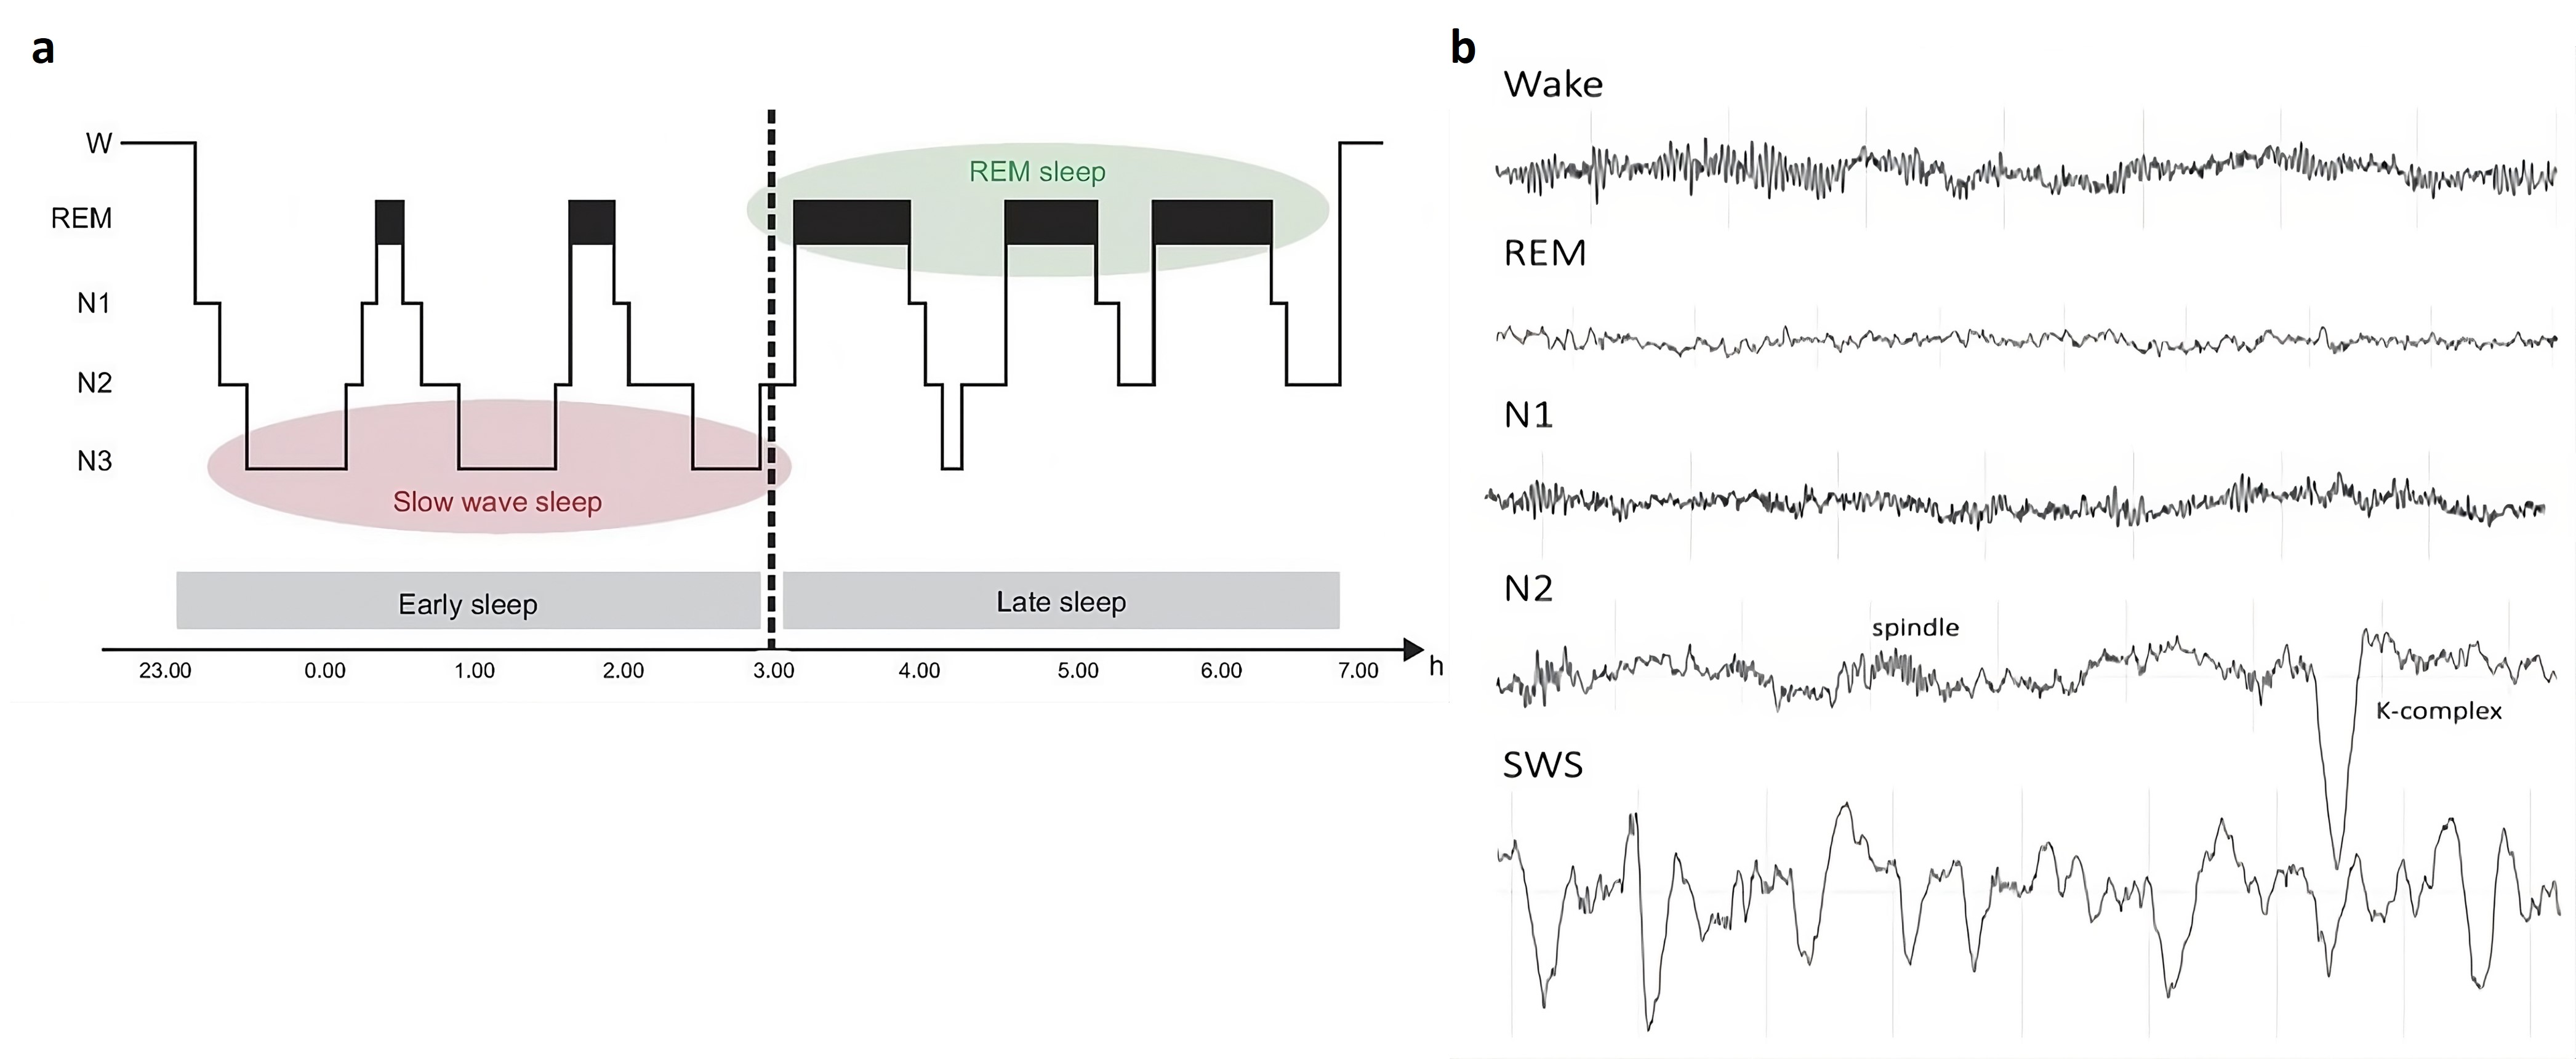
\includegraphics[width=0.9\linewidth]{1_Introduction/IntroImages/Picture1.jpg}
    \caption[\textit{Sleep architecture and oscillatory patterns.}]{\textit{Sleep architecture and oscillatory patterns.} \textbf{(a)} Hypnogram. Human sleep alternates in cycles between non-rapid eye movement (NREM) sleep and rapid eye movement (REM) sleep. Stages 3 and 4 of NREM are jointly referred to as slow wave sleep (SWS). Earlier periods of sleep are rich in SWS, whereas later periods contain greater amounts of REM sleep. Figure adapted from \cite{rasch_about_2013}. \textbf{(b)} Exemplary EEG traces for wake and each of the sleep stages. K-complexes and sleep spindles are key features of stage 2 of NREM sleep, while slow oscillations and delta waves prevail during SWS. \vspace{1cm} \label{fig:SleepPhysio}}
\end{figure}
 \FloatBarrier

The two major sleep stages that can be distinguished are Rapid Eye Movement (REM) sleep and Non-Rapid Eye Movement (NREM) sleep. The latter can be further subdivided into four stages: the lighter sleep stages 1 and 2, and the deeper sleep stages 3 and 4, now jointly referred to as slow wave sleep \parencite[SWS;][]{iber_aasm_2007}. NREM and REM sleep alternate or “cycle” across the night approximately every 90 minutes. Within each cycle, the ratio of NREM to REM varies throughout the night: NREM sleep predominates during the first half of the night, but as the night progresses, the length of REM periods becomes longer (see hypnogram in Figure \ref{fig:SleepPhysio}a). 

When transitioning from wakefulness to sleep, people typically spend a short period in Stage 1 of NREM sleep. This stage only accounts for up to 10\% of the total sleep time (TST) and is characterised by low-amplitude mixed-frequency activity (2-7 Hz) and less than 50\% of the wake-like alpha rhythm \parencite[8-13 Hz;][]{moser_sleep_2009, silber_visual_2007}. Sharply contoured waves called vertex sharp waves and slow rolling eye movements can also be observed \parencite{silber_visual_2007}. 

Stage 1 of NREM is typically followed by Stage 2, which takes up approximately 45–55\% of the TST. As shown in Figure \ref{fig:SleepPhysio}b, sleep spindles and K-complexes are the two pronounced oscillatory events that characterise this sleep stage (however, spindles can be also found during deeper sleep stages). \\
Sleep spindles are waxing and waning bursts of high-frequency activity that last about 0.5 to 3 seconds. They are generated in the thalamic reticular nucleus and then propagated into cortical regions through thalamocortical projections \parencite{de_gennaro_sleep_2003}. Their exact frequency range is still being debated; however, spindles are generally considered to be in the 10–15 Hz range and often further divided into slow spindles (< 13 Hz), which predominate in frontal cortices, and fast (> 13 Hz) spindles, which predominate in centroparietal areas \parencite{andrillon_sleep_2011,de_gennaro_sleep_2003,fernandez_sleep_2020,schabus_hemodynamic_2007,ulrich_sleep_2016}. Sleep spindles are primarily associated with memory consolidation, learning, and intellectual abilities \parencite{fernandez_sleep_2020,ulrich_sleep_2016}. For instance, evidence of their involvement in memory consolidation comes from a study conducted by Schabus and colleagues in which participants performed a declarative word-pair association task. Overnight change, computed as the number of recalled words in the evening after learning minus the number of recalled words in the morning after the intervening night, correlated significantly with increased spindle activity \parencite{schabus_sleep_2004}. Similarly, Morin and colleagues trained participants on a motor sequence task and retested their performance the following morning after a night of sleep. Both the number and duration of sleep spindles were higher in post-training sleep \parencite{morin_motor_2008}. In addition to the above-mentioned functions, sleep spindles have also been linked to plastic neuronal modifications, sleep protection against environmental disturbances, and cognitive dysfunction \parencite{astori_manipulating_2013,bergmann_local_2008,rasch_about_2013}.\\
K-complexes represent the largest event in a healthy human EEG. They have a widespread brain topography, although their maximal amplitude is typically frontal. K-complexes consist of high amplitude waves, made up of a negative sharp wave followed by a longer-lasting positive component; a shorter positivity precedes the negative wave but it is not easily discernible by eyes \parencite{colrain_k-complex_2005,ioannides_emergence_2019}. Functionally, k-complexes are believed to serve a sleep-protecting mechanism and a “sentinel” function that (1) evaluates the salience and/or alarm of internal and external signals; (2) promotes sleep maintenance; (3) suppresses cortical arousal; (4) promotes wakefulness \parencite{ioannides_emergence_2019,jahnke_wake_2012}. Additionally, they are considered a physiological correlate of arousal, as evidenced by their association with typical signs of arousal such as increases in heart rate and blood pressure, and respiratory shifts \parencite{forget_role_2011}.

Sleep deepens further into SWS which makes up 15-20\% of TST in young adults (this percentage decreases with aging). SWS is defined by the presence of four oscillatory rhythms: slow (SOs, 0.5-1 Hz) and delta oscillations (1-4 Hz), whose combined denomination is Slow Wave Activity (SWA, 0.5-4 Hz; see Figure \ref{fig:SleepPhysio}b), spindles (10-15 Hz) and ripples \parencite{iber_aasm_2007}. SOs, in addition to their low frequency, have a large peak-to-peak amplitude of at least 75 \(\mu\)V and an average peak-to-peak duration of 1 s. SOs are considered to be the pacemaker of brain activity during sleep, as they comprise a DOWN or hyperpolarization state and a UP or depolarisation state that reflects synchronous alterations in the membrane potential of neocortical neurons. SOs DOWN states are associated with neuronal silence, whereas SOs UP states with vigorous wake-like neuronal firing; both states last a few hundred milliseconds \parencite{massimini_sleep_2004,molle_fast_2011,nir_regional_2011}.
The other two prominent oscillations that characterise SWS are spindles - also present in S2 and discussed above - and sharp wave-ripples (SW-Rs). SW-Rs are composed of ripples and sharp waves. Sharp waves are fast depolarizing events generated in the CA3 region of the hippocampus, on which ripples are superimposed. Ripples are rapid bursts of elevated (100-300 Hz) neuronal activity generated in the CA1 region of the hippocampus \parencite{buzsaki_hippocampal_1986, rasch_about_2013}. Evidence suggests that these waves contribute to various aspects of memory, such as memory consolidation and retrieval \parencite{buzsaki_hippocampal_1986}.\\
SWS has been linked to both cognitive and physiological functions \parencite{leger_slow-wave_2018}. While SWS’s cognitive functions will be discussed later in more detail (see section \ref{Intro:sec:Models of sleep and memory}), it is worth mentioning its involvement in several important physiological activities. SWS supports the immune system’s response to infection by producing pro-inflammatory cytokines \parencite{lange_effects_2010} and plays a role in clearing metabolic waste, such as \(\beta\)-amyloid \parencite{leger_slow-wave_2018}. Moreover, SWS is associated with glucose regulation and the release and regulation of hormones. Regarding the former, a study conducted in young healthy adults showed that SWS deprivation resulted in a significant reduction of glucose tolerance and an increase in type 2 diabetes risk \parencite{tasali_sciences_2008}. Regarding the latter, there is evidence for a reduced release of growth hormone being linked to SWS deprivation \parencite[e.g.,][]{van_cauter_metabolic_2008}.

The last sleep stage is REM sleep, which when discovered in 1953 contradicted the general impression of sleep as a passive state \parencite{aserinsky_regularly_1953}. In fact, REM sleep, which accounts for ~25\% of TST, is also referred to as \textit{paradoxical sleep} because it displays EEG activity that closely resembles wakefulness with oscillations predominantly within the theta (4-7 Hz) and gamma (25-80 Hz) band ranges \parencite{iber_aasm_2007,steriade_synchronization_1996}. Moreover, REM sleep is characterized by skeletal muscle atonia (very low muscle tone) visible in the EMG, peripheral muscle twitches, and pronounced fluctuations in temperature and cardio-respiratory rhythms \parencite{peever_biology_2017}. REM sleep is composed of two different microstates, namely phasic and tonic periods. Tonic REM is considered to be a quiescent period in between periods of phasic activity characterized by ponto-geniculo-occipital (PGO) waves, bursts of eye movements (EM), sawtooth waves, myoclonic twitches and periods of marked respiratory and heart rate irregularities \parencite{simor_microstructure_2020}. REM sleep has been shown to be involved in the formation and consolidation of memories, such as procedural \parencite{peigneux_learned_2003}, declarative \parencite{fogel_dissociable_2007} and emotional \parencite{helm_overnight_2010} memories. Furthermore, it has also been involved in the reorganization of synaptic plasticity in the cortex \parencite{almeida-filho_memory_2018, pereira_differing_2020,zhou_rem_2020}. However, even though REM was discovered more than 60 years ago, evidence regarding its specific functions and mechanisms remain rather elusive although a consistent amount of evidence is provided by animal studies \parencite[e.g.,][]{peever_biology_2017, rasch_about_2013,simor_microstructure_2020}. For instance, PGO waves, bursts of large electric potentials that originate in the pons and propagate in the lateral geniculate nucleus and occipital cortex cannot be identified on a human scalp EEG, therefore they have been extensively studied in cats, rats, and primates \parencite{gott_towards_2017}. These waves, together with theta waves, have been proposed as a mechanism of synaptic plasticity \parencite{rasch_about_2013}.

As previously mentioned, NREM and REM sleep cycle throughout the night, with NREM sleep being more prevalent in the early part of the night. This pattern is explained by the theoretical model of sleep and wake regulation proposed by Borbely \parencite{borbely_two_1982,borbely_two-process_2016}. In this model, the interaction between the homeostatic sleep pressure (Process S) and the circadian pacemaker, an internal body clock operating on an approximately 24-hour rhythm (Process C), is key. The longer one stays awake, the more homeostatic sleep pressure accumulates, influencing the duration of SWS during the subsequent sleep period. This pressure diminishes throughout the sleep cycle, leading to a higher proportion of SWS shortly after sleep onset when the pressure is at its peak. Furthermore, these two processes are crucial in determining the quality and timing of sleep onset and offset. The influence of external stimuli, particularly light, plays a significant role in this context: the duration and timing of light exposure can lead to either a phase advance, shifting the circadian rhythm to an earlier time, or a phase delay, shifting it to a later time. Consequently, light exposure can affect various aspects of sleep, including its duration, timing, structure, and quality. This interplay between light, sleep patterns, and circadian rhythms is not only fundamental to understanding sleep itself but also has implications for learning and memory, which will be explored in more detail in Chapter 2. 


\section{Sleep and memory}\label{Intro:sec:Sleep and memory}
Of the many advantages conferred by sleep, this thesis will primarily examine sleep’s impact on memory. To provide context, an overview of memory systems and processes will be provided. The subsequent discussion will delve into the crucial role that sleep plays in memory, citing prominent theories that support this claim.

\subsection{Memory systems}
The notion that memory is not a single entity has been acknowledged for a long time. However, the first empirical evidence to support this idea was presented by Brenda Milner in 1957 through her study of the patient H.M., who underwent a bilateral resection of the medial temporal lobe to treat intractable epilepsy. Surprisingly, after the surgery, he was still able to learn new tasks, such as hand-eye coordination, even though he had no recollection of previous learning experiences \parencite{squire_conscious_2015}. This finding indicated that memory is not confined to a single structure but is instead composed of multiple systems that rely on different neuroanatomical structures. A comprehensive overview of the various types of memory has been reported by Henke \parencite{henke_model_2010} and it is depicted in Figure \ref{fig:LTM}. 

\FloatBarrier
\begin{figure}
    \centering    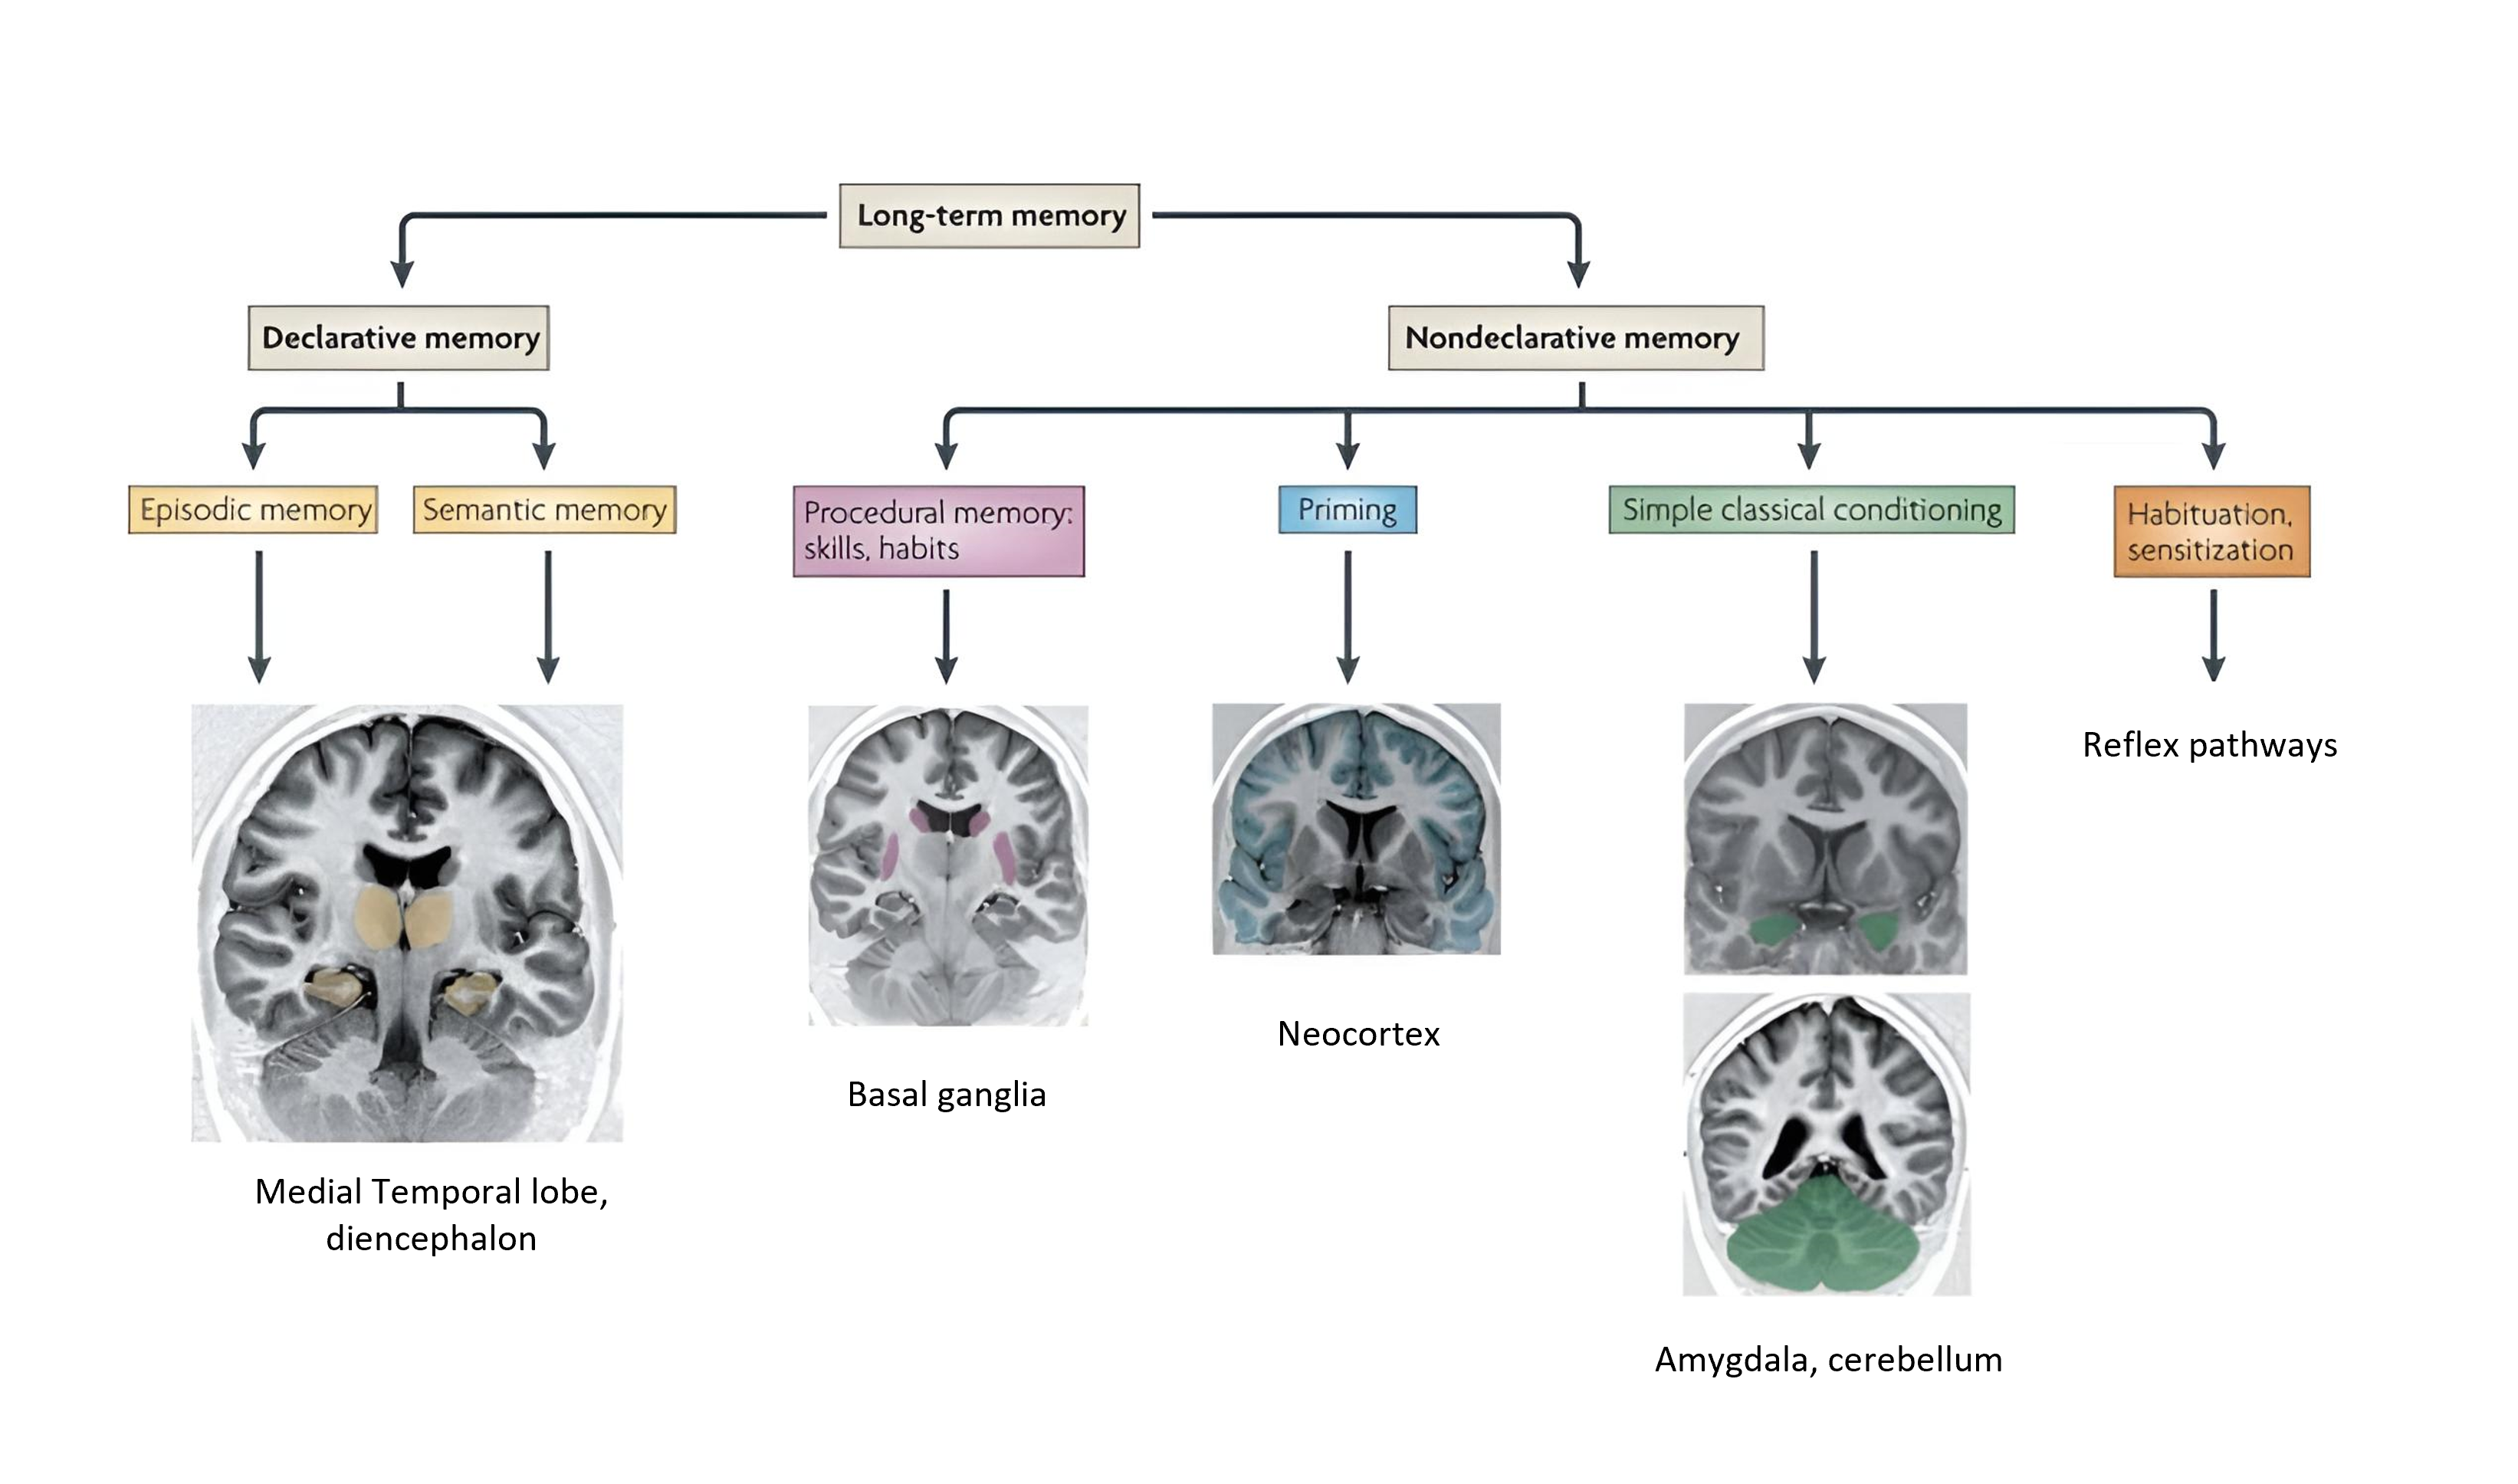
\includegraphics[width=0.9\linewidth]{1_Introduction//IntroImages/LTM.jpg}
    \caption[\textit{Organisation of long-term memory systems and associated brain structures}]{\textit{Organisation of long-term memory systems and associated brain structures.} Modified from \cite{henke_model_2010}. \vspace{1cm}}
    \label{fig:LTM}
\end{figure}

\FloatBarrier

The above figure illustrates the categorization of long-term memory into two primary types: declarative (explicit) and nondeclarative (implicit) memory \parencite{henke_model_2010,squire_conscious_2015,squire_structure_1996}. Declarative memory refers to the conscious recollection of information, and it can be further subdivided into memories for facts (semantic memory) and memories for events (episodic memory). Semantic memory refers to memories of information stored in the absence of contextual knowledge, whereas episodic memory is embedded in a specific spatiotemporal context. Non-declarative memories are instead linked to unconscious learning and retrieval capacities, and they can be classified into several subtypes. \\
The first subtype, procedural memories, refers to the learning of skills, such as riding a bike or playing an instrument; the second, priming, involves performance enhancement due to prior exposure to related information; the third, conditioning, involves the association of two unrelated stimuli to learn a new response; and finally, non-associative learning refers to the attenuation or augmentation of a response towards a repeated presentation of a stimulus \parencite{henke_model_2010,rasch_about_2013,squire_conscious_2015,squire_structure_1996}. The integrity of the medial temporal lobe system, which includes the hippocampus and entorhinal, perirhinal, and parahippocampal cortices, is thought to be essential for declarative memories. In contrast, nondeclarative memories are generally considered to be hippocampus-independent \parencite{squire_conscious_2015,squire_structure_1996}.
\FloatBarrier



\subsection{Memory processes}\label{Intro:sec:Memory processes}
Memory is formed over time through three distinct processes: encoding, consolidation, and retrieval. 
Encoding comprises the formation of new memory traces following the perception of a stimulus. These newly encoded traces are initially labile and susceptible to chance and forgetting, but they become increasingly robust and resistant to interference through consolidation. During this process, the new memory traces are integrated into pre-existing long-term memory networks \parencite{rasch_about_2013}.

\textit{Consolidation} involves two steps: synaptic and system consolidation. The initial step is accomplished at a synaptic level within minutes or hours after learning and leads to enduring changes in synaptic connections \parencite{kandel_molecular_2001}. Synaptic consolidation is then supplemented by system consolidation which redistributes synaptic connectivity across different brain areas \parencite{frankland_organization_2005}. These changes enable the newly encoded information to become part of long-term memory, providing a basis for later retrieval \parencite{rasch_about_2013}. However, two significant challenges arise: how newly learned material becomes permanently accessible without overwriting old memories, and how the brain determines what information to store or forget. 

The \textbf{standard two-stage model of memories} \parencite{marr_simple_1971} offered a solution to the first issue, and nowadays, it constitutes the most influential model of human memory. The model suggests that effective learning requires two complementary systems: the hippocampus and the neocortex. During wakefulness, the hippocampus acts as a fast-learning storage where new memory traces are temporarily stored. These memories are gradually transferred into the neocortex, a long-term slow-learning storage system. The model further proposes that the transfer process (from the short-term store to the long-term one) occurs slowly via repeated and spontaneous reactivation of hippocampal-cortical networks. Over time, network reactivation increases the stability and strength of cortico-cortical connections, allowing integration of the traces into pre-existing neocortical knowledge networks. Ultimately, this results in memories becoming hippocampal-independent \parencite{frankland_organization_2005,marr_simple_1971,squire_retrograde_1995}. These complementary memory systems allow the storage of new memories without interfering with existing ones.

With respect to the second challenge - how the brain determines what information to store or forget - it seems sensible that information in some way relevant for adapting to the environment or important for upcoming challenges will be preferred. In this context, emotions have been shown to play a significant role in labelling which information will be stored in memory and which will be forgotten \parencite{dolan_emotion_2002,williams_power_2022}. Numerous studies have demonstrated that emotional stimuli are better remembered than their neutral counterparts, largely due to the modulatory role played by the amygdala in the process of hippocampal-dependent memory formation \parencite{anderson_neural_2003,mcgaugh_memory_2000,mcgaugh_role_2002,vuilleumier_effects_2001,whalen_masked_1998}. Indeed, during the initial encoding phase, the amygdala rapidly responds to emotional stimuli, often before conscious awareness, thereby enhancing attention to prioritise the processing of these stimuli. In later stages of memory formation, it modulates the effects of stress hormones in the consolidation of hippocampal-dependent memories \parencite{diano_amygdala_2017,phelps_human_2004}. As a result, emotionally charged events are more readily remembered. 

The hippocampo-cortical information transfer of memories is a continuous process that occurs not only during wakefulness but also during offline periods including sleep. Sleep, indeed, is an ideal time window for these processes to occur as it protects memories from interference by preventing encoding of new information \parencite{ellenbogen_role_2006,rasch_about_2013}.
\FloatBarrier



\subsection{Models of sleep and memory}\label{Intro:sec:Models of sleep and memory}
Although as early as 1885 Ebbinghaus published a seminal study demonstrating the effect of time on forgetting (i.e. forgetting is reduced when followed by a period of sleep), the interest in studying the relationship between sleep and memory was reignited only in the late 1980s with a variety of studies demonstrating the beneficial effects of NREM and REM sleep on memory consolidation \parencite[see][for a review]{rasch_about_2013}. A differential role of these two sleep stages in the consolidation of different types of memory was theorised by the \textbf{Dual Process Hypothesis} \parencite{gais_declarative_2004,rasch_about_2013,smith_sleep_2001}. This account assumes that hippocampus-dependent declarative memories are linked to NREM sleep, while REM sleep benefits the consolidation of nondeclarative memories, such as procedural and emotional. The Dual process hypothesis is supported by human studies that employed the “night–half paradigm”, in which participants’ memory performance is compared across retention intervals including the early half (rich in NREM sleep) and the late half of the night (rich in REM sleep). However, this methodology overlooks the fact that neither the early nor the late half of the night contains one stage of sleep. Furthermore, subsequent experiments have not consistently demonstrated this distinction \parencite[e.g.,][]{fogel_dissociable_2007,huber_arm_2006,rauchs_consolidation_2004}, and theoretical accounts have proposed that the cyclic succession of NREM and REM sleep may constitute the key to successful overnight memory consolidation. 

The \textbf{Sequential hypothesis} \parencite{ambrosini_learning_2001,giuditta_sequential_1995} stresses this concept and assumes that during SWS, non-adaptive or irrelevant memory traces are downscaled (or eliminated), while useful memories are strengthened. Subsequently, during REM sleep, these adaptive memories are integrated with pre-existing memories. Supporting evidence for the Sequential hypothesis has been originally obtained from studies conducted with animals \parencite[e.g.,][]{ambrosini_sequential_1992,ambrosini_sequential_1995} and then confirmed in humans \parencite[e.g.,][]{ficca_morning_2000,mednick_sleep-dependent_2003,stickgold_visual_2000}. For example, Ficca and colleagues investigated the impact of sleep cycle disorganisation on the recall of verbal material in young adults and demonstrated that morning recall was significantly affected by sleep cycle disorganisation \parencite{ficca_morning_2000}.

The \textbf{Active System Consolidation Hypothesis} \parencite[ASC,][Figure \ref{fig:ASC}]{diekelmann_memory_2010,rasch_about_2013} represents the most prominent model in the field. It originates from the Standard two-stage model of memories (see section \ref{Intro:sec:Memory processes}) and argues that sleep is not merely a passive state but is actively involved in memory consolidation. Furthermore, central to this model is the concept that newly encoded memory representations are repeatedly reactivated during sleep, a vital process for consolidation. During encoding, labile memory traces are stored temporarily in the hippocampus. Subsequently, during SWS, these traces undergo repeated reactivation, facilitating their gradual transfer to the cortex for long-term storage (Figure \ref{fig:ASC}A). The involvement of SWS in memory processing is well-documented \parencite{diekelmann_memory_2010, walker_role_2009, rasch_about_2013}, highlighting its importance in this model.
A critical aspect of the transfer of memory traces involves the precise temporal synchronization of three key oscillations during SWS: neocortical slow oscillations, thalamo-cortical spindles, and hippocampal sharp wave ripples (Figure \ref{fig:ASC}B). The SOs up-states trigger memory reactivations in tandem with hippocampal ripples. Ripples have been shown to occur in the troughs of spindles, which are in turn coupled with the SOs up-states. This intricate coupling is essential for the efficient transfer of reactivated memory traces, thereby facilitating their integration into the neocortex \parencite{rasch_about_2013}. 

\FloatBarrier
\begin{figure}
    \centering
    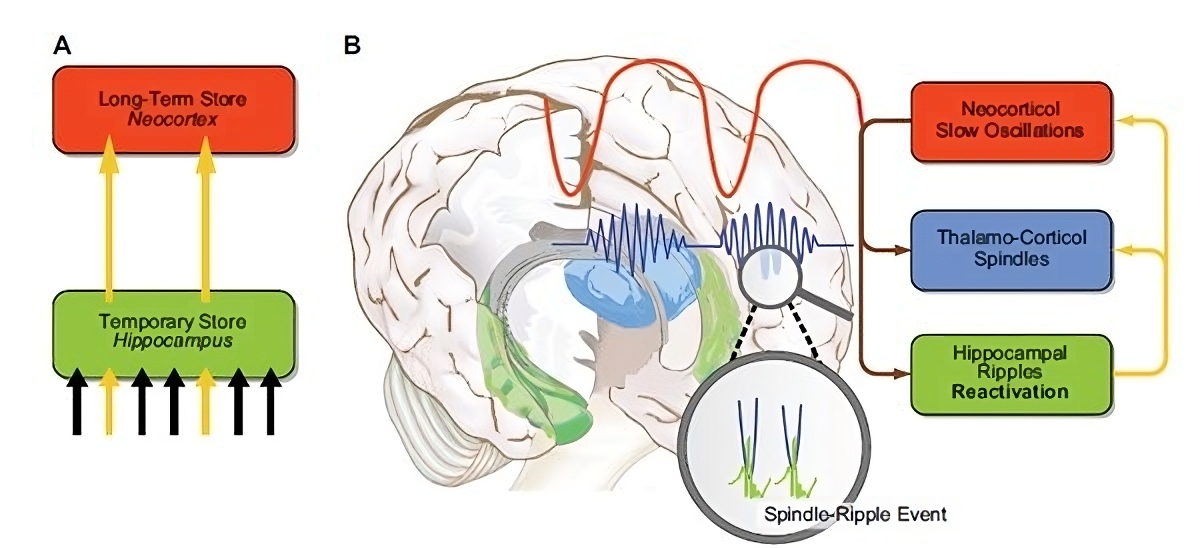
\includegraphics[width=0.9\linewidth]{1_Introduction//IntroImages/Picture4-K7_mBWyR6-transformed.jpeg}
    \caption[\textit{The Active System Consolidation Hypothesis}]{\textit{The Active System Consolidation Hypothesis.} \textbf{(A)} Newly acquired memories are encoded into a temporary store, the hippocampus, and transferred to the long-term neocortical store during SWS. \textbf{(B)} The cortico-hippocampal dialogue is orchestrated by neocortical slow oscillations (red), thalamo-cortical spindles (blue), and hippocampal sharp-wave ripples (green). Source: \cite{rasch_about_2013}. \vspace{1cm}}
    \label{fig:ASC}
\end{figure}
\FloatBarrier

The hypothesis further suggests that the temporal synchronization of SWS-related oscillations not only supports memory reactivation but also leads to a qualitative reorganization of memories, involving their redistribution and transformation. Additionally, REM sleep contributes to the stabilization of these transferred memories through synaptic consolidation. Empirical evidence from various studies bolsters this hypothesis. For example, research in rodents using paradigms like fear conditioning or object recognition tasks has demonstrated the necessity of this coupling for effective consolidation \parencite{maingret_hippocampo-cortical_2016, latchoumane_thalamic_2017}. Similarly, human intracranial EEG recordings in epilepsy patients have corroborated these findings \parencite{helfrich_bidirectional_2019, jiang_posterior_2019}. Finally, the coupling between SOs and spindles was shown to correlate with performance improvements on several memory tasks \parencite[for instance][]{schreiner_endogenous_2021, muehlroth_precise_2019, hahn_slow_2020}.

An alternative hypothesis for the mechanisms underlying memory consolidation during sleep has been offered by the \textbf{Synaptic Homeostasis Hypothesis} \parencite[SHY,][Figure \ref{fig:SHY}]{tononi_sleep_2003,tononi_sleep_2006}. It postulates that wakefulness is accompanied by a net increase in synaptic strength that progressively saturates learning abilities. Sleep, as an antidote, promotes synaptic downscaling, renormalizing the net synaptic strength and restoring the brain’s ability for future encoding (synaptic homeostasis), while maintaining certain memory traces. Further, this renormalization mechanism is proposed to occur during SWA, a hallmark of SWS. This hypothesis has been corroborated by sleep deprivation studies that demonstrated that memory performance is worse after waking than sleep \parencite{ashton_sleep_2020, gais_sleep_2006, yang_repeated_2012} and by studies that highlighted that the amount of SWA predicts memory performance after sleep \parencite{huber_arm_2006, ferrarelli_increase_2019}.
Crucially, SHY suggests that memories tagged as important are weakened less - or relatively strengthened - overnight than irrelevant memories, thus promoting the consolidation and integration of memories \parencite{tononi_sleep_2003,tononi_sleep_2006,tononi_sleep_2014, wilhelm_sleep_2014}.

\FloatBarrier
\begin{figure}
    \centering
    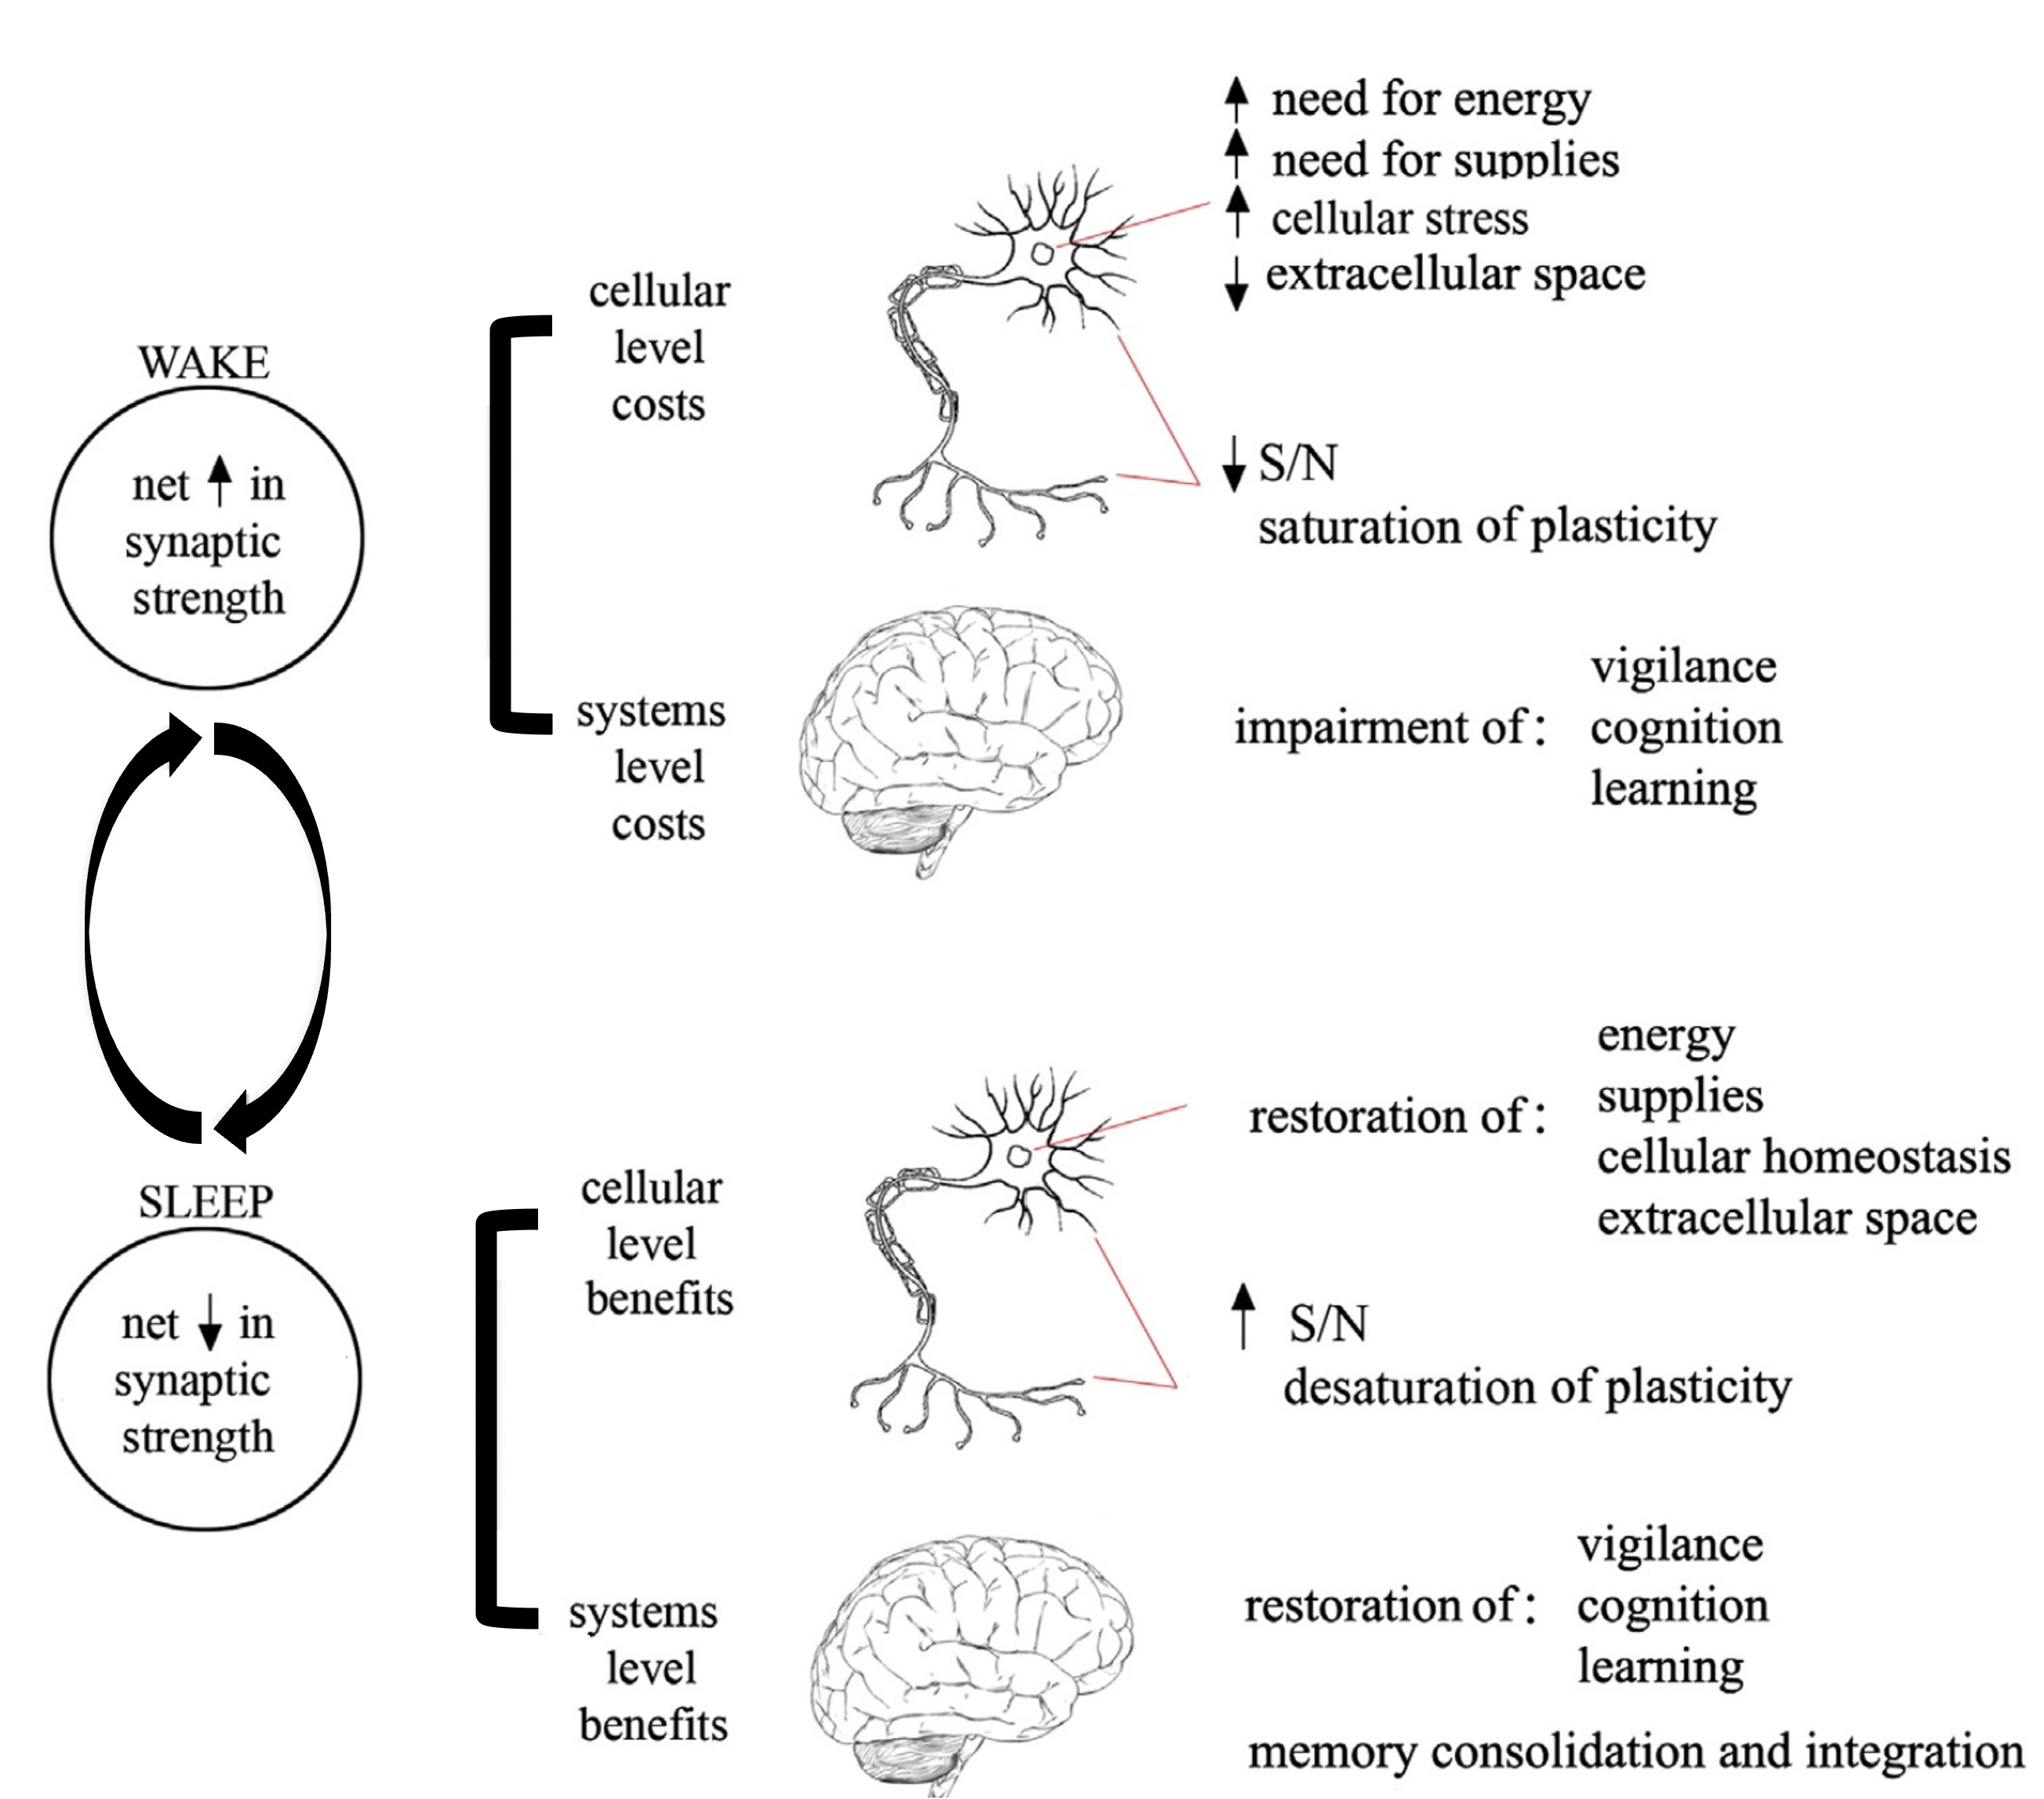
\includegraphics[width=0.8\linewidth]{1_Introduction//IntroImages/Picture5.jpg}
    \caption[\textit{Synaptic Homeostasis Hypothesis}]{\textit{Synaptic Homeostasis Hypothesis.} Modified from \cite{tononi_sleep_2014}. \vspace{0.8cm}}
    \label{fig:SHY}
\end{figure}
\FloatBarrier

There is evidence of a more rapid transfer of information from the hippocampus to the neocortex if the new set of information to be acquired is compatible (overlaps) with an existing framework of organised knowledge, called \textit{schema} \parencite{tse_schemas_2007,van_kesteren_persistent_2010,van_kesteren_retrieval_2010}. The \textbf{Information overlap to abstract} (iOtA) model developed by Lewis and Durrant explains the underlying mechanisms of this facilitation effect and the role sleep plays in it \parencite{lewis_overlapping_2011}. The model states that during SWS, the replay of overlapping memories is strengthened through Hebbian plasticity, representing the core mechanism for schema formation. Synaptic interconnections between neurons that code for shared elements are strengthened and survive SWS downscaling \parencite{abbott_synaptic_2000,lewis_overlapping_2011, tononi_sleep_2003,tononi_sleep_2006}. Thereby, only newly learned information that overlaps with an existing schema and is reactivated on multiple occasions will be potentiated and incorporated into the schema. The replay of overlapping memories in SWS leads to the extraction of commonalities or ‘gist’ (the core of a memory), promoting both a quantitative and a qualitative reorganisation of memory representations \parencite{durrant_sleep-dependent_2011,ellenbogen_human_2007,lewis_overlapping_2011}. The iOtA model is the foundation of the \textbf{Broader Form of the iOtA Model} \parencite[BiOtA]{lewis_how_2018}, which integrates REM sleep into the framework. The BiOtA model emphasizes the significance of the cyclic structure of a night’s sleep, in which NREM and REM alternate. During NREM sleep, the replay of thematically related memories is enhanced, while during REM sleep, the connections between seemingly disparate concepts are recognised, resulting in the formation of new connections between concepts \parencite[Figure \ref{fig:biota};][]{lewis_how_2018}. The interleaving of these two stages could explain the role of sleep in creativity and problem-solving. 
\vspace{1cm}
\begin{figure}[H]
    \centering
    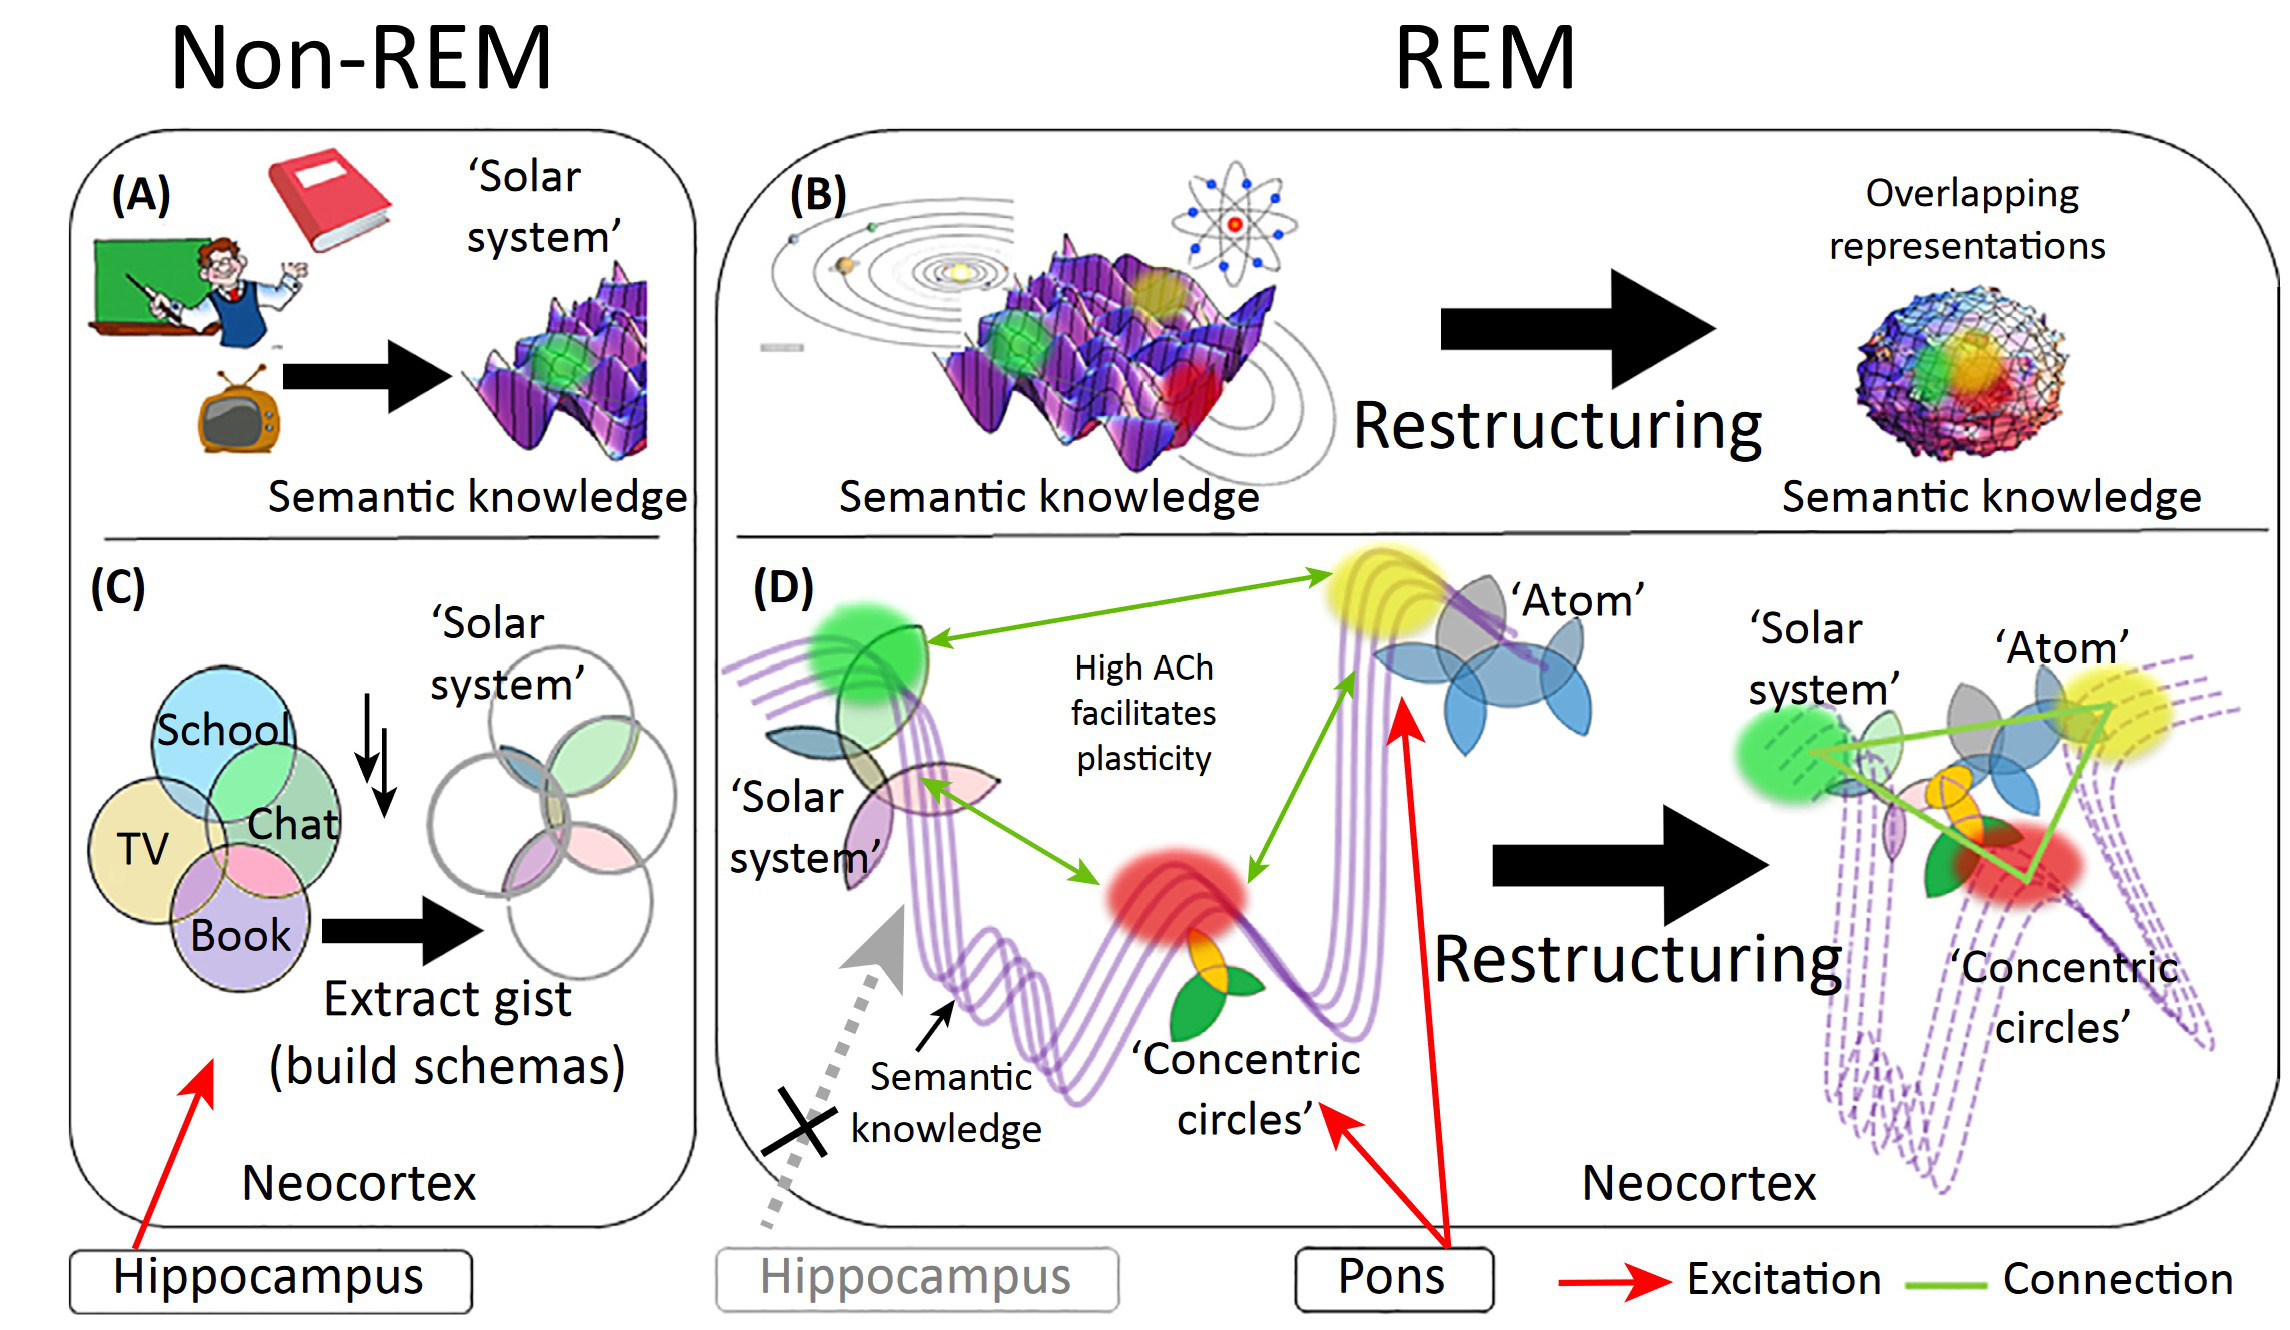
\includegraphics[width=0.9\linewidth]{1_Introduction//IntroImages/Picture6.jpg}
    \caption[\textit{The BiOtA model.}]{\textit{The BiOtA model.} \textbf{A} and \textbf{B} provide a simpler representation of \textbf{C} and \textbf{D}. \textbf{(A-C)} During NREM sleep, overlapping memories are replayed in the neocortex. Areas of overlap are strengthened, leading to general abstraction or the formation of new schemas. \textbf{(B-D)} During REM sleep, connections between the hippocampus and the neocortex are lost, and PGO waves trigger activity in other schemas, allowing the detection of similarities between schemas that, once found, lead to the restructure of knowledge. Modified from \cite{lewis_how_2018}.\vspace{1cm}}
    \label{fig:biota}
\end{figure}
\FloatBarrier

Finally, as briefly mentioned in Section \ref{Intro:sec:Memory processes}, a substantial body of research suggests that emotional memories are preferentially consolidated across sleep \parencite{alger_preferential_2018,cairney_targeted_2014,cunningham_psychophysiological_2014,groch_role_2013,hu_sleep_2006,nishida_rem_2009,tempesta_emotional_2015,wagner_brief_2006,wagner_emotional_2001}; however, see \parencite{lipinska_preferential_2019} that challenges this view. According to the \textbf{Sleep to Forget, Sleep to Remember Hypothesis} (SFSR), while the content (the information) of emotional memories is strengthened over time, the affective responses associated with their recall are attenuated across multiple nights of sleep \parencite{helm_overnight_2010,walker_role_2009}. It is therefore possible that time plays a vital role in modulating sleep’s impact on the visceral charge (emotional strength) of emotional memories. Moreover, the SFSR hypothesis also suggests that REM sleep, because of its unique biology, represents a particular brain state for the consolidation and modulation of emotional memories, and a variety of studies have confirmed this hypothesis \parencite{groch_role_2013,groch_dissociating_2015,harrington_influence_2018,helm_overnight_2010,hutchison_targeted_2021,nishida_rem_2009,menz_role_2013,menz_rem_2016,payne_sleep_2012,wagner_emotional_2001,wagner_brief_2006,wassing_restless_2019}.
Indeed, during REM sleep we observe (1) increased activity in limbic and paralimbic structures, which are key brain regions involved in the formation and consolidation of emotional memories; (2) theta oscillations, which propagation in limbic and prefrontal regions are believed to modulate affective experiences in both animals and humans; (3) increased concentrations of acetylcholine (ACh) - crucial for the long-term consolidation of emotional learning - and reduced concentration of noradrenergic and serotonergic input to the cortex, associated with lower levels of stress and anxiety \parencite[see] [for reviews]{walker_role_2009, helm_overnight_2010}.
\FloatBarrier


\section{Memory reactivation}\label{Intro:sec:Memory reactivation}
Before diving into different studies conducted on animals and humans on memory reactivation, it is crucial to clarify some technical terms. Genzel and colleagues provided definitions to facilitate the use of a common language among researchers \parencite{genzel_consensus_2020}. As per their definitions, the term reactivation refers to the re-emergence of a previously encoded pattern at a later point in time, whereas replay directly assesses the temporal structure of the sequential information \parencite{genzel_consensus_2020}. This terminology will be used throughout the thesis. 

\subsection{Animal studies}
The first evidence of spontaneous memory replay during sleep is found in the rodent literature on place cells. Place cells are hippocampal CA1 pyramidal neurons that fire selectively when the animal occupies a specific location in the environment, known as place fields \parencite{girardeau_hippocampal_2011,okeefe_hippocampus_1971}. By following the sequence of place cells, the rat’s movements from one location to another can be traced. 
Pavlides and Winson demonstrated that during subsequent sleeping states, hippocampal place cells used in recent awake exploration exhibited an increased firing rate compared to cells that were not involved in the pre-sleep exploration \parencite{pavlides_influences_1989}. In the seminal study by Wilson and McNaughton, the activity of pairs of hippocampal place cells was recorded during both a spatial navigation task in a maze and during the SWS period that preceded and followed the task \parencite{wilson_reactivation_1994}. Notably, during the SWS period that followed the task, the same place cells that fired during exploratory behaviour fired together, indicating that information acquired during active behaviour is re-expressed in hippocampal circuits during sleep. The order of neuronal firing observed during wakefulness was preserved during sleep reactivation, albeit in a compressed temporal manner \parencite{wilson_reactivation_1994}. \\
Reactivation during sleep has also been observed in various brain regions and species, thereby supporting the Active System Consolidation Hypothesis (see section \ref{Intro:sec:Models of sleep and memory}). For instance, visual \parencite{ji_coordinated_2007}, parietal \parencite{qin_memory_1997}, prefrontal \parencite{benchenane_coherent_2010,euston_fast-forward_2007,johnson_stored-trace_2010,peyrache_replay_2009} and sensorimotor cortices \parencite{hoffman_coordinated_2002} have all shown reactivation. 
Evidence of reactivation and replay during REM sleep is substantially less extensive compared to NREM, however the occurrence of these phenomena in rodents is supported by place cell recordings \parencite{louie_temporally_2001,poe_experience-dependent_2000}, appetitive conditioning \parencite{maho_appetitive_2002} and cell recording from the primary motor cortex \parencite{eckert_neural_2020}.
Interestingly, while replay during NREM sleep occurs in a temporally compressed form \parencite{lee_memory_2002}, REM sleep replay is temporally structured at a timescale closer to that seen during wakefulness \parencite{louie_temporally_2001}. Just like replay during sleep, wake replay is triggered by SW-Rs however, the order during awake replay is reversed compared to that seen during sleep  \parencite{foster_reverse_2006}. 





\subsection{Human studies}
Studies investigating memory reactivation during sleep in humans are limited due to the low temporal and spatial resolution of non-invasive techniques compared to electrophysiological recordings \parencite{schreiner_electrophysiological_2020}. 
Early attempts to reveal memory reactivation during sleep in humans, investigated whether brain regions activated during memory encoding show corresponding activity during subsequent sleep \parencite{bergmann_sleep_2012,maquet_experience-dependent_2000,peigneux_are_2004,yotsumoto_location-specific_2009}. For instance, using simultaneous EEG-fMRI recordings Bergmann and colleagues observed that participants who learned face-scene associations exhibited increased activity in both hippocampal and neocortical areas compared to those who performed a visuomotor control task. The increased neural activation was temporally coupled with increased spindle amplitude and correlated with pre-sleep behavioural performance, indicating the involvement of spindles in reactivation-like patterns \parencite{bergmann_sleep_2012}. Another study employed positron emission topography (PET) to investigate the effects of training on a probabilistic serial reaction time task. Findings indicated that brain areas activated during the task in wakefulness were similarly active during REM after the training, thus supporting the hypothesis that there is an experience-dependent re-activation of specific brain areas during post-training REM sleep \parencite{maquet_experience-dependent_2000}.
The advent of multivariate pattern analysis \parencite[MVPA;][]{haxby_distributed_2001} and representational similarity analysis \parencite[RSA;][]{schonauer_decoding_2017} helped tackle the issue of whether the re-expression of encoding related activity reflects the content of the learned task. In other words, studies that used these techniques aimed to measure replay of stimulus-related activity patterns \parencite{deuker_memory_2013,liu_human_2019,schonauer_decoding_2017,sterpenich_memory_2014,zhang_electrophysiological_2018}. For instance, Schönauer and colleagues used MVPA to decode EEG activity during sleep to determine whether participants viewed faces or houses during a declarative task performed the day before. They showed that the memory content was reprocessed during both NREM and REM sleep and that reactivation of declarative material during NREM sleep was associated with a greater memory performance \parencite{schonauer_decoding_2017}. Furthermore, combining intracranial EEG electrodes with RSA in epilepsy patients, Zhang and colleagues identified that stimulus-specific activity spontaneously re-occurred during waking rest and sleep, but only ripple-triggered replay during NREM sleep was associated with memory consolidation \parencite{zhang_electrophysiological_2018}.\\
These studies support the evidence that the spontaneous reactivation of prior learned material during sleep constitutes a plausible mechanism supporting sleep-based memory consolidation. However, only methods that can directly manipulate memory reactivation during sleep provide evidence for a causal role of sleep in memory consolidation. Targeted Memory Reactivation (TMR) is a technique that emerged to directly address this issue.




\subsection{Targeted Memory Reactivation (TMR)}
TMR involves associating learning materials used in a task during awake learning with a contextual cue, like a sound or an odour. These stimuli are then unobtrusively re-presented during sleep, usually during specific sleep stages, to bias the spontaneous memory reactivation process towards the cued stimuli.  Performance change scores between reactivated and non-reactivated items are then compared during a post-sleep test. The aim of this technique is to selectively improve memory consolidation of the cued items and thereby increase performance on those items in subsequent memory tests \parencite{andrillon_sleep_2011,hu_promoting_2020,rasch_odor_2007}.
Early attempts with the use of TMR date back to the end of the 1980s \parencite{oudiette_upgrading_2013}, however, this procedure was experimentally demonstrated for the first time by Rasch and colleagues in 2007 \parencite{rasch_odor_2007}. In this seminal study, olfactory stimuli were used to cue declarative memory during sleep. Participants were trained on a two-dimensional memory task involving object locations while smelling the scent of a rose. During the subsequent night, the same odour was presented again during SWS periods without disrupting participants’ sleep. Declarative memory improvement was measured the next day by comparing the recall performance of participants who did or did not receive the rose-scented air during sleep. Those who received the TMR procedure demonstrated enhanced recall performance for the cued stimuli compared to a control group. Additionally, functional magnetic resonance imaging (fMRI) revealed a higher hippocampal activation for those object-location pairs that were re-exposed to the odour during SWS \parencite{oudiette_upgrading_2013,rasch_odor_2007}. However, it remained unclear from this study whether TMR during sleep has the ability to selectively reactivate and strengthen specific memories formed during a learning episode. \\
Rudoy and colleagues \parencite{rudoy_strengthening_2009} addressed the specificity issues by using auditory cues instead of sounds. Participants learned semantic associations between images and sounds (e.g., cat/meow) in specific locations. During the TMR procedure delivered during SWS, half of the items were cued by representing the sound of the corresponding objects. Post-sleep results showed higher accuracy for the items that were cued during sleep, suggesting that specific memories can be targeted and strengthened during sleep \parencite{rudoy_strengthening_2009}. \\
These findings have been further supported by animal studies. Bendor and Wilson trained four rats on an auditory-spatial association task in which sounds (sound L or R) were associated with reward locations: rats received a food pellet reward at the left-end side of a track for sound L and at the right-end side for sound R. In addition, control sounds not associated with the behavioural task were also played. During subsequent sleep, auditory cues were represented during NREM sleep, and place cell activity in the CA1 region of the hippocampus was recorded during the task and during sleep. After comparing firing rates for each acoustic stimulus during NREM periods, they observed that both task-related cues (sound L and R) biased the content of replay events. Sound L resulted in a higher firing rate of individual place cells and ensembles of place cells with place fields on the left side, while sound R had the same effect on the right side \parencite{bendor_biasing_2012}.

TMR has been applied during both NREM (N2 and SWS) and REM sleep however, to date, a relatively low number of studies examined the effect of TMR during REM sleep. The majority of studies applied TMR during SWS to boost performance on declarative memory tasks. Beyond spatial location \parencite{diekelmann_labile_2011,diekelmann_offline_2012,rasch_odor_2007,rudoy_strengthening_2009}, TMR studies have shown a benefit for spatial navigation \parencite{shimizu_closed-loop_2018}, vocabulary learning \parencite{schreiner_boosting_2015}, associative learning tasks \parencite{cairney_mechanisms_2017,cairney_memory_2018}, word recall \parencite{fuentemilla_hippocampus-dependent_2013}. Additionally, evidence shows that SWS TMR can improve non-declarative memories such as procedural skills \parencite{antony_cued_2013,cousins_cued_2014,cousins_cued_2016,schonauer_strengthening_2013} and emotional memories \parencite{cairney_targeted_2014,lehmann_emotional_2016,hu_promoting_2020}.\\
TMR during N2 has been mainly employed with motor skill learning tasks \parencite{laventure_nrem2_2016,laventure_beyond_2018} due to the well-known role played by sleep spindles in the consolidation of motor memories traces \parencite{fogel_function_2011,morin_motor_2008}. 
Not many TMR studies focused on REM sleep. Early studies conducted with animals, by Hennevin and Hars, reported significant performance improvement in rats on an active avoidance conditioning task after receiving ear shocks as a cue during post-learning REM sleep \parencite{hars_improvement_1985,hennevin_is_1987}. Early attempts in humans also demonstrated enhanced memory after auditory stimulation during REM on a Morse code task \parencite{guerrien_enhancement_1989} and a complex logic task \parencite{smith_post_1990}. On the contrary, more recent attempts have reported negative REM sleep-declarative and procedural memory effects \parencite{laventure_nrem2_2016,rasch_odor_2007} and a positive REM-emotional memory effect \parencite{hutchison_targeted_2021,schwartz_enhancing_2022,wassing_restless_2019}.\\
Today’s research takes advantage of artificial intelligence methods to develop automated sleep stage scoring and to perform TMR in participants’ own homes, thus allowing real-life applications. Recently, Whitmore and colleagues developed a TMR system called “SleepStim” that works with a smartphone and a smartwatch used to play sounds and record movement and heart rate parameters, respectively \parencite{whitmore_improving_2022}. They tested whether at-home TMR, delivered via the SleepStim system during N3, replicates the spatial-memory benefit observed in laboratory settings. Across two experiments, they found a stronger TMR effect using a relatively low auditory cue intensity \parencite{whitmore_improving_2022}. Furthermore, TMR manipulations can be extended to clinical settings and used in clinical psychotherapy. Some studies explored the potential of TMR to weaken fear memories \parencite{hauner_stimulus-specific_2013,oudiette_fear_2014} and to reduce negative valence of stimuli \parencite{hutchison_targeted_2021,rihm_replay_2015}, which could be used to treat emotion and memory-related disorders, such as depression and PTSD. For example, a clinical reduction in nightmare frequency and more positive dream emotions have been demonstrated in adults with nightmare disorder (ND) after exposing them to TMR during REM sleep for 14 days in combination with imagery rehearsal therapy \parencite{schwartz_enhancing_2022}. 

\subsection{Research objectives}
This thesis comprises three experimental chapters that investigate the beneficial effects of sleep manipulation on cognition. 

\textbf{Chapter 2 }aimed to examine whether blocking natural light during nighttime sleep with the use of an eye mask benefits memory and alertness. To this end, we compared participants’ performance on a cognitive battery while wearing an eye mask or a control mask during sleep. Additionally, we utilised a wearable EEG device to track sleep architecture, as we were interested in looking at the impact of the eye mask manipulation on sleep parameters.

\textbf{Chapter 3} explored the role of sleep in consolidating the effects of a cognitive training, thereby overcoming functional fixedness, a cognitive obstacle that prevents people from thinking outside the box and reaching insight. Participants were first exposed to a training session and then their performance was compared after a period of nocturnal sleep or daytime wakefulness. 

In \textbf{Chapter 4}, the focus switched to assessing the potential of TMR during REM sleep to disarm the effects of negative emotions. We examined the effect of cueing on subjective and objective measurement of arousal. To this end, we employed subjective ratings of arousal, functional MRI, and heart rate deceleration.  





\newpage
\thispagestyle{empty}



\newpage
%\thispagestyle{plain}
\mbox{}
\newpage

% 2nd Chapter
%\include{2_Chapter/main_chapter_2}
%\newpage
%\thispagestyle{plain}
%\mbox{}
%\newpage

% 3rd Chapter
%\include{3_Chapter/main_chapter_3}
%\newpage
%\thispagestyle{plain}
%\mbox{}
%\newpage

% 4th Chapter
%\include{4_Chapter/main_chapter_4}
%\newpage
%\thispagestyle{plain}
%\mbox{}
%\newpage

% Conclusion
%\include{5_General Discussion/ConclusionMain}
%\newpage
%\mbox{}
%\newpage
%\backmatter


\printbibliography[heading=bibintoc]
\end{document}
